\documentclass{article}
%%%%%%%%%%%%%%%%%%%%%%%%%%%%% Define Article %%%%%%%%%%%%%%%%%%%%%%%%%%%%%%%%%%
%%%%%%%%%%%%%%%%%%%%%%%%%%%%%%%%%%%%%%%%%%%%%%%%%%%%%%%%%%%%%%%%%%%%%%%%%%%%%%%

%%%%%%%%%%%%%%%%%%%%%%%%%%%%% Using Packages %%%%%%%%%%%%%%%%%%%%%%%%%%%%%%%%%%
\usepackage{float}
\usepackage[letterpaper,portrait]{geometry}
\usepackage{graphicx}
\usepackage{anysize}
\usepackage{lipsum}
\usepackage{amsmath,amssymb,amsthm}
\usepackage[utf8]{inputenc}
\usepackage{multirow}
\usepackage{csquotes}
\usepackage[spanish]{babel}
\usepackage{apacite}
\usepackage{multicol}
\usepackage{parskip}
\usepackage{setspace}
\usepackage{empheq}
\usepackage{mdframed}
\usepackage{booktabs}
\usepackage{lipsum}
\usepackage{graphicx}
\usepackage{color}
\usepackage{psfrag}
\usepackage{pgfplots}
\usepackage{bm}
\usepackage{tocloft}
\usepackage{lscape}
\usepackage{adjustbox}
\setlength{\tabcolsep}{1.505625pt}
\renewcommand{\arraystretch}{1.2}
%%%%%%%%%%%%%%%%%%%%%%%%%%%%%%%%%%%%%%%%%%%%%%%%%%%%%%%%%%%%%%%%%%%%%%%%%%%%%%%

% Other Settings

%%%%%%%%%%%%%%%%%%%%%%%%%% Page Setting %%%%%%%%%%%%%%%%%%%%%%%%%%%%%%%%%%%%%%%
\geometry{letterpaper, margin=2.54cm}

%%%%%%%%%%%%%%%%%%%%%%%%%% Define some useful colors %%%%%%%%%%%%%%%%%%%%%%%%%%
\definecolor{ocre}{RGB}{243,102,25}
\definecolor{mygray}{RGB}{243,243,244}
\definecolor{deepGreen}{RGB}{26,111,0}
\definecolor{shallowGreen}{RGB}{235,255,255}
\definecolor{deepBlue}{RGB}{61,124,222}
\definecolor{shallowBlue}{RGB}{235,249,255}
%%%%%%%%%%%%%%%%%%%%%%%%%%%%%%%%%%%%%%%%%%%%%%%%%%%%%%%%%%%%%%%%%%%%%%%%%%%%%%%

%%%%%%%%%%%%%%%%%%%%%%%%%% Define an orangebox command %%%%%%%%%%%%%%%%%%%%%%%%
\newcommand\orangebox[1]{\fcolorbox{ocre}{mygray}{\hspace{1em}#1\hspace{1em}}}
%%%%%%%%%%%%%%%%%%%%%%%%%%%%%%%%%%%%%%%%%%%%%%%%%%%%%%%%%%%%%%%%%%%%%%%%%%%%%%%

%%%%%%%%%%%%%%%%%%%%%%%%%%%% English Environments %%%%%%%%%%%%%%%%%%%%%%%%%%%%%
\newtheoremstyle{mytheoremstyle}{3pt}{3pt}{\normalfont}{0cm}{\rmfamily\bfseries}{}{1em}{{\color{black}\thmname{#1}~\thmnumber{#2}}\thmnote{\,--\,#3}}
\newtheoremstyle{myproblemstyle}{3pt}{3pt}{\normalfont}{0cm}{\rmfamily\bfseries}{}{1em}{{\color{black}\thmname{#1}~\thmnumber{#2}}\thmnote{\,--\,#3}}
\theoremstyle{mytheoremstyle}
\newmdtheoremenv[linewidth=1pt,backgroundcolor=shallowGreen,linecolor=deepGreen,leftmargin=0pt,innerleftmargin=20pt,innerrightmargin=20pt,]{theorem}{Theorem}[section]
\theoremstyle{mytheoremstyle}
\newmdtheoremenv[linewidth=1pt,backgroundcolor=shallowBlue,linecolor=deepBlue,leftmargin=0pt,innerleftmargin=20pt,innerrightmargin=20pt,]{definition}{Definition}[section]
\theoremstyle{myproblemstyle}
\newmdtheoremenv[linecolor=black,leftmargin=0pt,innerleftmargin=10pt,innerrightmargin=10pt,]{problem}{Problem}[section]
%%%%%%%%%%%%%%%%%%%%%%%%%%%%%%%%%%%%%%%%%%%%%%%%%%%%%%%%%%%%%%%%%%%%%%%%%%%%%%%

%%%%%%%%%%%%%%%%%%%%%%%%%%%%%%% Plotting Settings %%%%%%%%%%%%%%%%%%%%%%%%%%%%%
\usepgfplotslibrary{colorbrewer}
\pgfplotsset{width=8cm,compat=1.9}
%%%%%%%%%%%%%%%%%%%%%%%%%%%%%%%%%%%%%%%%%%%%%%%%%%%%%%%%%%%%%%%%%%%%%%%%%%%%%%%

%%%%%%%%%%%%%%%%%%%%%%%%%%%%%%% Title & Author %%%%%%%%%%%%%%%%%%%%%%%%%%%%%%%%
\author{Gustavo Vergara}
%%%%%%%%%%%%%%%%%%%%%%%%%%%%%%%%%%%%%%%%%%%%%%%%%%%%%%%%%%%%%%%%%%%%%%%%%%%%%%%

\begin{document}
\pgfplotsset{compat=1.18}
\setstretch{2}

\begin{titlepage}
	\centering
	\vspace{2.5cm}
	{\scshape \Large TALLER DE CARTAS POR ATRIBUTOS\par}
	\vspace{5cm}
	\textbf\large\scshape{\par}
	\vspace{0.5cm}
	{\Large Vergara Pareja Gustavo\par}
	\vspace{5cm}
	{\scshape\Large Miguel Ángel Lancheros\par}
	\vspace{0.3cm}
	{\scshape\Large Metrología y Control de Calidad - G1IM \par}
	\vspace{0.3cm}
	{\scshape\Large Universidad de Córdoba\par}
	\vspace{0.3cm}
	{\Large 6 de Diciembre de 2023 \par}
\end{titlepage}
\tableofcontents
\newpage
\section{Introducción}
\begin{itemize}
	\item Cualquier característica de calidad que pueda ser clasificada de forma binaria: “cumple o no
	cumple”, “funciona o no funciona”, “pasa o no pasa”, “conforme o disconforme” “defectuoso,
	no defectuoso”, será considerado como un atributo y para su control se utilizan Cartas de Control por Atributos.
	En el caso de las cartas para variables, tenemos dos cartas, una para la tendencia central y otra
	para la dispersión. En el control por atributos, tanto la media como la variabilidad de la
	proporción muestral dependen de un único parámetro, por lo que se hace sólo una carta de control.
	Existen diferentes tipos de cartas de control por atributos sin embargo solo estudiaremos las
	siguientes: Cartas P, NP, y U.
\end{itemize}
\section{Carta de control por atributos P (Proporción de defectuosos)}
	\begin{itemize}
		\item Estas cartas miden la proporción de unidades no conformes en un grupo de unidades que se
		inspecciona. El objetivo es comprobar si la evolución de las proporciones muestrales observadas
		son compatibles con un mismo valor poblacional p.
		Este tipo de grafica se puede construir con n constante o variable por lo que a continuación se
		muestra el procedimiento para ambos casos.
		\begin{figure}[!ht]
			\centering
			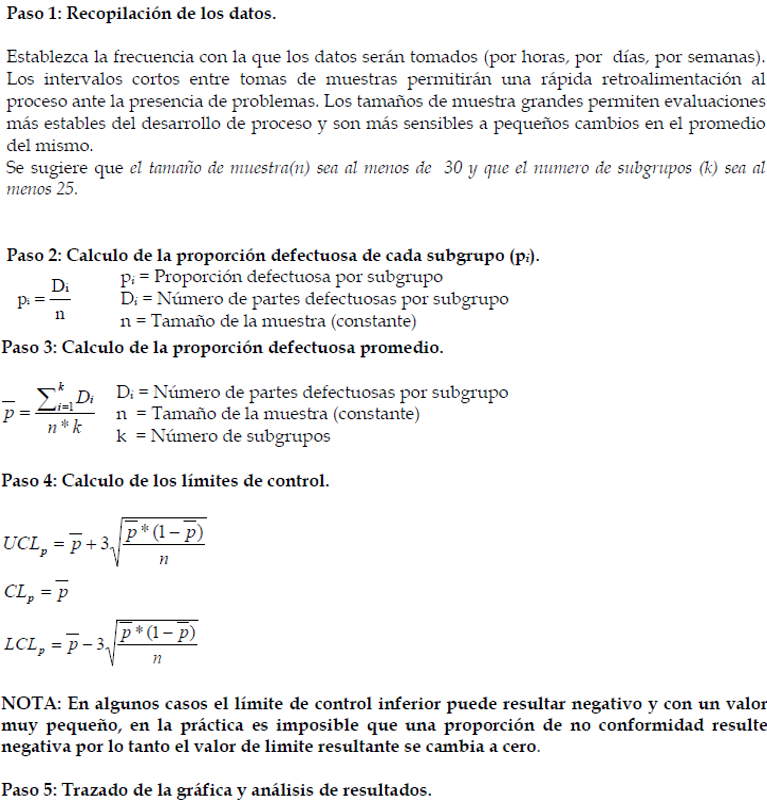
\includegraphics[width=0.6\textwidth]{CartaPVar.png}
			\caption[short]{Pasos para Carta P, con n constante}
			\label{fig:imagen2}
		  \end{figure}
		\begin{figure}[H]
			\centering
			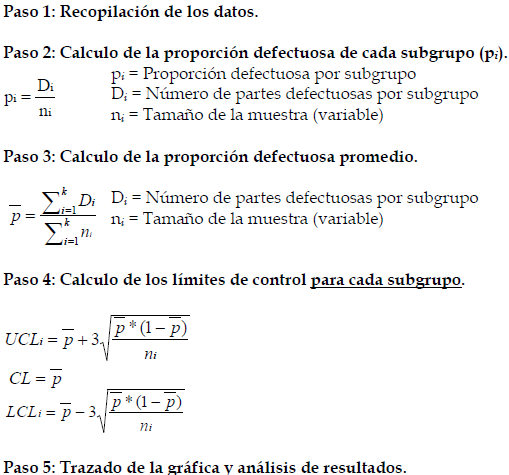
\includegraphics[width=0.6\textwidth]{CartaP.png}
			\caption[short]{Pasos para Carta P, con n variable}
			\label{fig:imagen2}
		  \end{figure}
	
	\end{itemize}
	Un fabricante de latas de aluminio registra el número de partes defectuosas, tomando
	muestras cada hora de 50 latas, con 30 subgrupos. Construir la carta de control p (proporción de
	defectuosos) para la siguiente serie de datos obtenida durante el muestreo además dar un
	informe de la interpretación de carta obtenida. (Construir una carta de control P)
	\begin{table}[ht!]
		\centering
		\begin{tabular}{|l|l|l|l|l|l|}
		\hline
			Subgrupo & Latas defectuosas & pi & UCL & CL & LCL \\ \hline
			1 & 12 & 0.24 & 0.410239119 & 0.231333333 & 0.052427548 \\ \hline
			2 & 15 & 0.3 & 0.410239119 & 0.231333333 & 0.052427548 \\ \hline
			3 & 8 & 0.16 & 0.410239119 & 0.231333333 & 0.052427548 \\ \hline
			4 & 10 & 0.2 & 0.410239119 & 0.231333333 & 0.052427548 \\ \hline
			5 & 4 & 0.08 & 0.410239119 & 0.231333333 & 0.052427548 \\ \hline
			6 & 7 & 0.14 & 0.410239119 & 0.231333333 & 0.052427548 \\ \hline
			7 & 16 & 0.32 & 0.410239119 & 0.231333333 & 0.052427548 \\ \hline
			8 & 9 & 0.18 & 0.410239119 & 0.231333333 & 0.052427548 \\ \hline
			9 & 14 & 0.28 & 0.410239119 & 0.231333333 & 0.052427548 \\ \hline
			10 & 10 & 0.2 & 0.410239119 & 0.231333333 & 0.052427548 \\ \hline
			11 & 5 & 0.1 & 0.410239119 & 0.231333333 & 0.052427548 \\ \hline
			12 & 6 & 0.12 & 0.410239119 & 0.231333333 & 0.052427548 \\ \hline
			13 & 17 & 0.34 & 0.410239119 & 0.231333333 & 0.052427548 \\ \hline
			14 & 12 & 0.24 & 0.410239119 & 0.231333333 & 0.052427548 \\ \hline
			15 & 22 & 0.44 & 0.410239119 & 0.231333333 & 0.052427548 \\ \hline
			16 & 8 & 0.16 & 0.410239119 & 0.231333333 & 0.052427548 \\ \hline
			17 & 10 & 0.2 & 0.410239119 & 0.231333333 & 0.052427548 \\ \hline
			18 & 5 & 0.1 & 0.410239119 & 0.231333333 & 0.052427548 \\ \hline
			19 & 13 & 0.26 & 0.410239119 & 0.231333333 & 0.052427548 \\ \hline
			20 & 11 & 0.22 & 0.410239119 & 0.231333333 & 0.052427548 \\ \hline
			21 & 20 & 0.4 & 0.410239119 & 0.231333333 & 0.052427548 \\ \hline
			22 & 18 & 0.36 & 0.410239119 & 0.231333333 & 0.052427548 \\ \hline
			23 & 24 & 0.48 & 0.410239119 & 0.231333333 & 0.052427548 \\ \hline
			24 & 15 & 0.3 & 0.410239119 & 0.231333333 & 0.052427548 \\ \hline
			25 & 9 & 0.18 & 0.410239119 & 0.231333333 & 0.052427548 \\ \hline
			26 & 12 & 0.24 & 0.410239119 & 0.231333333 & 0.052427548 \\ \hline
			27 & 7 & 0.14 & 0.410239119 & 0.231333333 & 0.052427548 \\ \hline
			28 & 13 & 0.26 & 0.410239119 & 0.231333333 & 0.052427548 \\ \hline
			29 & 9 & 0.18 & 0.410239119 & 0.231333333 & 0.052427548 \\ \hline
			30 & 6 & 0.12 & 0.410239119 & 0.231333333 & 0.052427548 \\ \hline
			~ & 347 & ~ & ~ & ~ & ~ \\ \hline
			~ & P & 0.231333333 \\ \hline
		\end{tabular}
	\end{table}
	\begin{figure}[ht!]
		\centering
		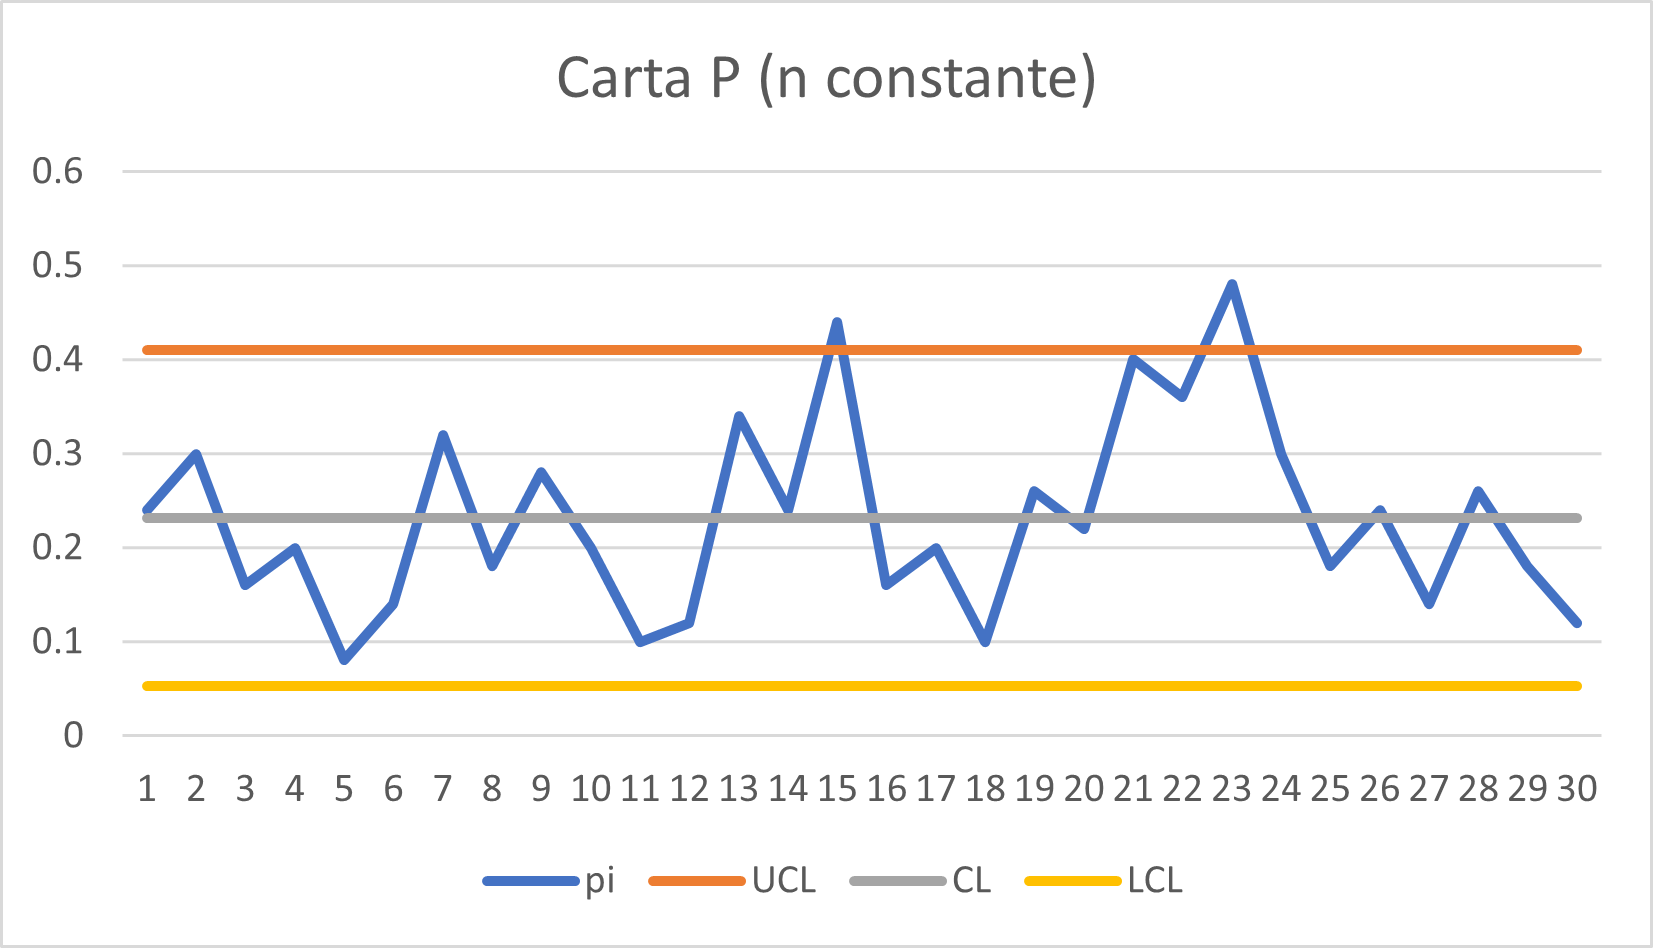
\includegraphics[width=0.6\textwidth]{GrafP.png}
		\caption[short]{Gráfico Carta P}
		\label{fig:imagen2}
	  \end{figure}
	  \newpage
\section{Carta de control por atributos NP (Número de defectuosos)}

\begin{itemize}
	\item La carta np es una herramienta estadística usada para evaluar el número de artículos
	defectuosos o el número de artículos no conformes producidos por un proceso. Tenga en cuenta
	que siempre que una carta np se pueda utilizar también se podrá utilizar una carta p.
	\begin{figure}[H]
		\centering
		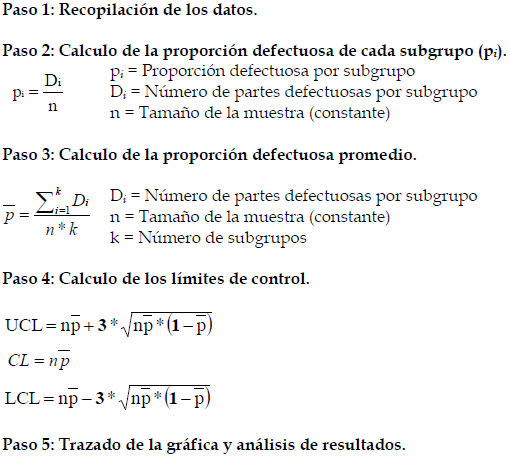
\includegraphics[width=0.6\textwidth]{CartaNP.png}
		\caption[short]{Pasos para Carta NP}
		\label{fig:imagen2}
	  \end{figure}
	\item La siguiente tabla de datos fue obtenida mediante la apertura al azar de una caja seleccionada
	de cada envío y contando el número de perfiles de acero golpeados que tenia cada caja. Había 250
	perfiles por caja.
	Construir una carta de control np (número de defectuosos).
\end{itemize}
\begin{table}[H]
    \centering
    \begin{tabular}{|l|l|l|l|l|l|}
    \hline
        No. de envío & Perfiles golpeados & pi & UCL & CL & LCL \\ \hline
        1 & 20 & 0.08 & 42.87690185 & 27.93333333 & 12.98976482 \\ \hline
        2 & 28 & 0.112 & 42.87690185 & 27.93333333 & 12.98976482 \\ \hline
        3 & 24 & 0.096 & 42.87690185 & 27.93333333 & 12.98976482 \\ \hline
        4 & 21 & 0.084 & 42.87690185 & 27.93333333 & 12.98976482 \\ \hline
        5 & 32 & 0.128 & 42.87690185 & 27.93333333 & 12.98976482 \\ \hline
        6 & 33 & 0.132 & 42.87690185 & 27.93333333 & 12.98976482 \\ \hline
        7 & 31 & 0.124 & 42.87690185 & 27.93333333 & 12.98976482 \\ \hline
        8 & 29 & 0.116 & 42.87690185 & 27.93333333 & 12.98976482 \\ \hline
        9 & 30 & 0.12 & 42.87690185 & 27.93333333 & 12.98976482 \\ \hline
        10 & 34 & 0.136 & 42.87690185 & 27.93333333 & 12.98976482 \\ \hline
        11 & 32 & 0.128 & 42.87690185 & 27.93333333 & 12.98976482 \\ \hline
        12 & 24 & 0.096 & 42.87690185 & 27.93333333 & 12.98976482 \\ \hline
        13 & 29 & 0.116 & 42.87690185 & 27.93333333 & 12.98976482 \\ \hline
        14 & 27 & 0.108 & 42.87690185 & 27.93333333 & 12.98976482 \\ \hline
        15 & 37 & 0.148 & 42.87690185 & 27.93333333 & 12.98976482 \\ \hline
        16 & 23 & 0.092 & 42.87690185 & 27.93333333 & 12.98976482 \\ \hline
        17 & 27 & 0.108 & 42.87690185 & 27.93333333 & 12.98976482 \\ \hline
        18 & 28 & 0.112 & 42.87690185 & 27.93333333 & 12.98976482 \\ \hline
        19 & 31 & 0.124 & 42.87690185 & 27.93333333 & 12.98976482 \\ \hline
        20 & 27 & 0.108 & 42.87690185 & 27.93333333 & 12.98976482 \\ \hline
        21 & 30 & 0.12 & 42.87690185 & 27.93333333 & 12.98976482 \\ \hline
        22 & 23 & 0.092 & 42.87690185 & 27.93333333 & 12.98976482 \\ \hline
        23 & 23 & 0.092 & 42.87690185 & 27.93333333 & 12.98976482 \\ \hline
        24 & 27 & 0.108 & 42.87690185 & 27.93333333 & 12.98976482 \\ \hline
        25 & 35 & 0.14 & 42.87690185 & 27.93333333 & 12.98976482 \\ \hline
        26 & 29 & 0.116 & 42.87690185 & 27.93333333 & 12.98976482 \\ \hline
        27 & 23 & 0.092 & 42.87690185 & 27.93333333 & 12.98976482 \\ \hline
        28 & 23 & 0.092 & 42.87690185 & 27.93333333 & 12.98976482 \\ \hline
        29 & 30 & 0.12 & 42.87690185 & 27.93333333 & 12.98976482 \\ \hline
        30 & 28 & 0.112 & 42.87690185 & 27.93333333 & 12.98976482 \\ \hline
        ~ & 838 & ~ & ~ & ~ & ~ \\ \hline
        ~ & P & 0.111733333 & ~ & ~ & ~ \\ \hline
    \end{tabular}
\end{table}
\begin{figure}[H]
	\centering
	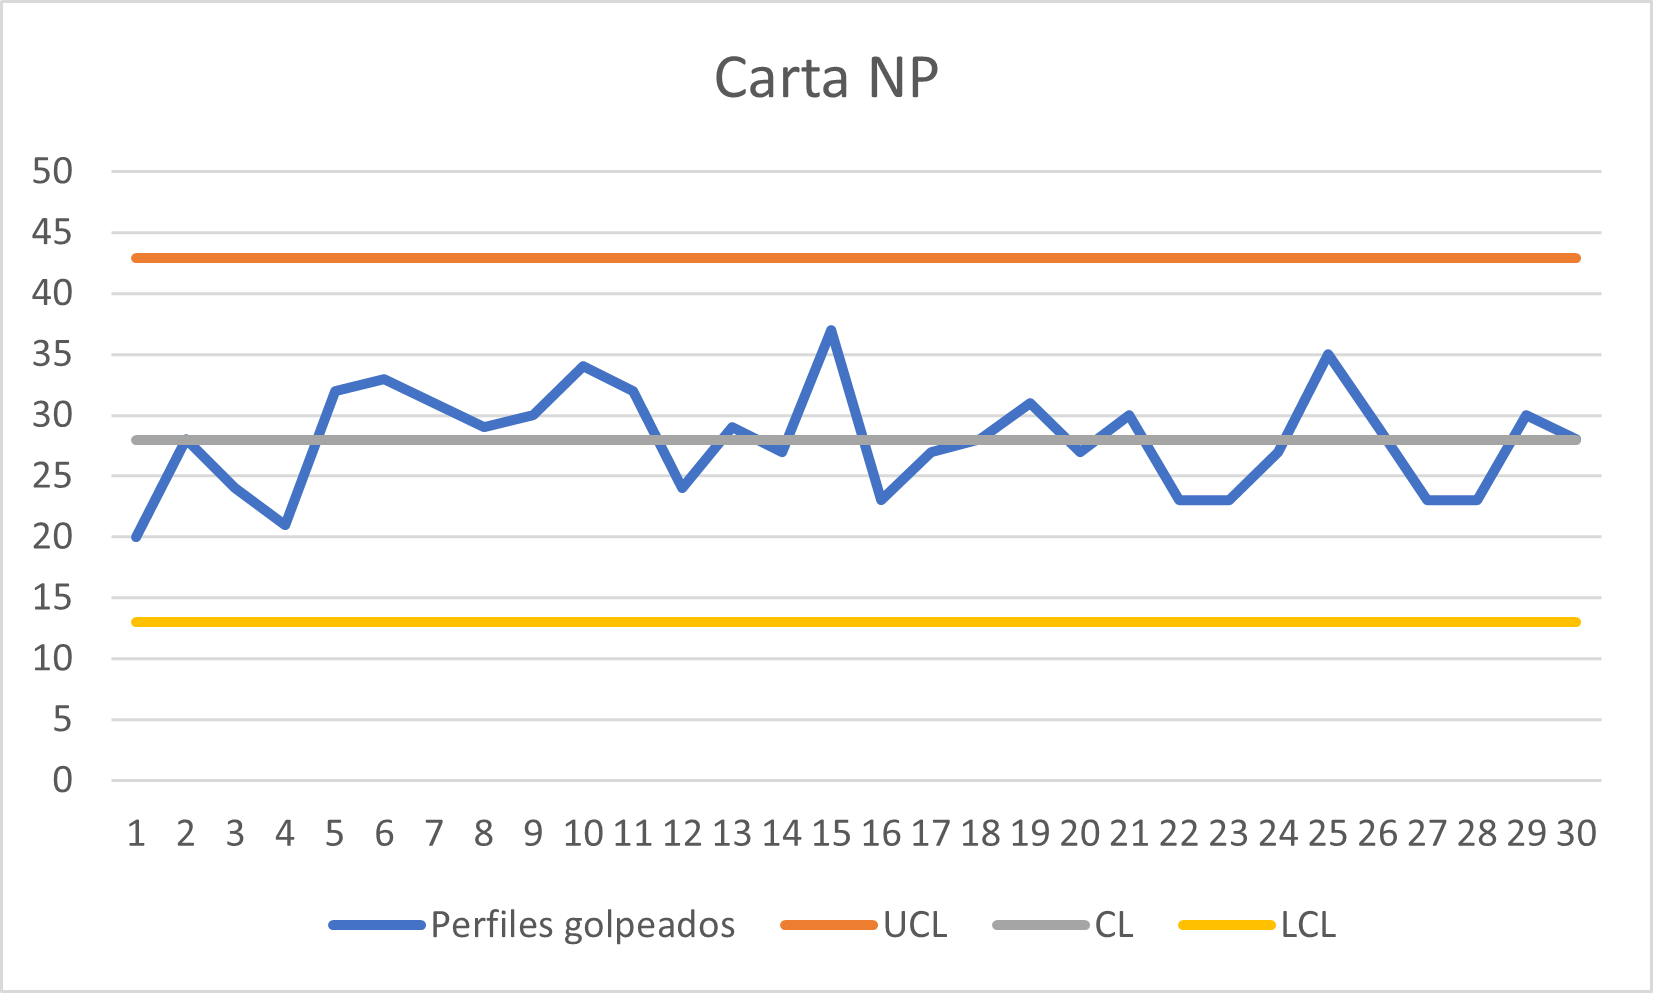
\includegraphics[width=0.6\textwidth]{GrafNP.png}
	\caption[short]{Gráfico Carta NP}
	\label{fig:imagen2}
  \end{figure}
\section{Carta de control por atributos U (Número de ocurrencias por unidad)}
\begin{itemize}
	\item La carta u es una herramienta estadística usada para evaluar la variación del número promedio
	de defectos por articulo o unidad. Se usa cuando el tamaño del subgrupo no es constante.
	\begin{figure}[H]
		\centering
		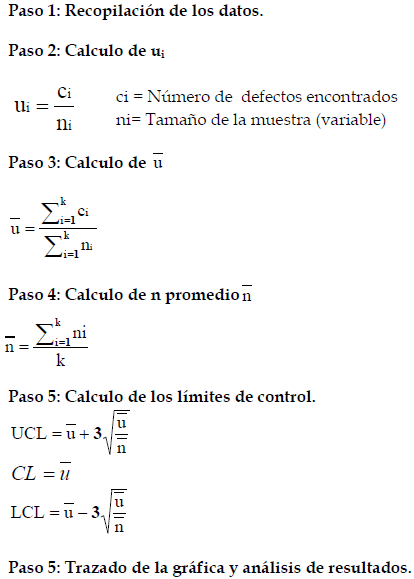
\includegraphics[width=0.6\textwidth]{CartaU.png}
		\caption[short]{Pasos para Carta U}
		\label{fig:imagen2}
	  \end{figure}
\end{itemize}	 
En una fábrica se ensamblan artículos electrónicos y al final del proceso se hace una
inspección por muestreo para detectar defectos relativamente menores. En la siguiente tabla se
presenta el número de defectos observados en muestreos realizados en 24 lotes consecutivos de
piezas electrónicas. Construir una carta de control U.
\begin{table}[!ht]
    \centering
    \begin{tabular}{|l|l|l|l|l|l|l|}
    \hline
        Lote & Tamaño de muestra & Detectos encontrados & Ui & UCL & CL & LCL \\ \hline
        1 & 20 & 17 & 0.85 & 1.701638622 & 1.045714286 & 0.38978995 \\ \hline
        2 & 20 & 24 & 1.2 & 1.701638622 & 1.045714286 & 0.38978995 \\ \hline
        3 & 20 & 16 & 0.8 & 1.701638622 & 1.045714286 & 0.38978995 \\ \hline
        4 & 20 & 26 & 1.3 & 1.701638622 & 1.045714286 & 0.38978995 \\ \hline
        5 & 15 & 15 & 1 & 1.701638622 & 1.045714286 & 0.38978995 \\ \hline
        6 & 15 & 15 & 1 & 1.701638622 & 1.045714286 & 0.38978995 \\ \hline
        7 & 15 & 20 & 1.333333333 & 1.701638622 & 1.045714286 & 0.38978995 \\ \hline
        8 & 25 & 18 & 0.72 & 1.701638622 & 1.045714286 & 0.38978995 \\ \hline
        9 & 25 & 26 & 1.04 & 1.701638622 & 1.045714286 & 0.38978995 \\ \hline
        10 & 25 & 10 & 0.4 & 1.701638622 & 1.045714286 & 0.38978995 \\ \hline
        11 & 25 & 25 & 1 & 1.701638622 & 1.045714286 & 0.38978995 \\ \hline
        12 & 30 & 21 & 0.7 & 1.701638622 & 1.045714286 & 0.38978995 \\ \hline
        13 & 30 & 40 & 1.333333333 & 1.701638622 & 1.045714286 & 0.38978995 \\ \hline
        14 & 30 & 24 & 0.8 & 1.701638622 & 1.045714286 & 0.38978995 \\ \hline
        15 & 30 & 46 & 1.533333333 & 1.701638622 & 1.045714286 & 0.38978995 \\ \hline
        16 & 30 & 32 & 1.066666667 & 1.701638622 & 1.045714286 & 0.38978995 \\ \hline
        17 & 30 & 30 & 1 & 1.701638622 & 1.045714286 & 0.38978995 \\ \hline
        18 & 30 & 34 & 1.133333333 & 1.701638622 & 1.045714286 & 0.38978995 \\ \hline
        19 & 15 & 11 & 0.733333333 & 1.701638622 & 1.045714286 & 0.38978995 \\ \hline
        20 & 15 & 14 & 0.933333333 & 1.701638622 & 1.045714286 & 0.38978995 \\ \hline
        21 & 15 & 30 & 2 & 1.701638622 & 1.045714286 & 0.38978995 \\ \hline
        22 & 15 & 17 & 1.133333333 & 1.701638622 & 1.045714286 & 0.38978995 \\ \hline
        23 & 15 & 18 & 1.2 & 1.701638622 & 1.045714286 & 0.38978995 \\ \hline
        24 & 15 & 20 & 1.333333333 & 1.701638622 & 1.045714286 & 0.38978995 \\ \hline
        ~ & 525 & 549 & ~ & ~ & ~ & ~ \\ \hline
        ~ & ~ & ~ & ~ & ~ & ~ & ~ \\ \hline
        ~ & U & 1.045714286 & ~ & ~ & ~ & ~ \\ \hline
        ~ & n & 21.875 \\ \hline
    \end{tabular}
\end{table}
\begin{figure}[H]
	\centering
	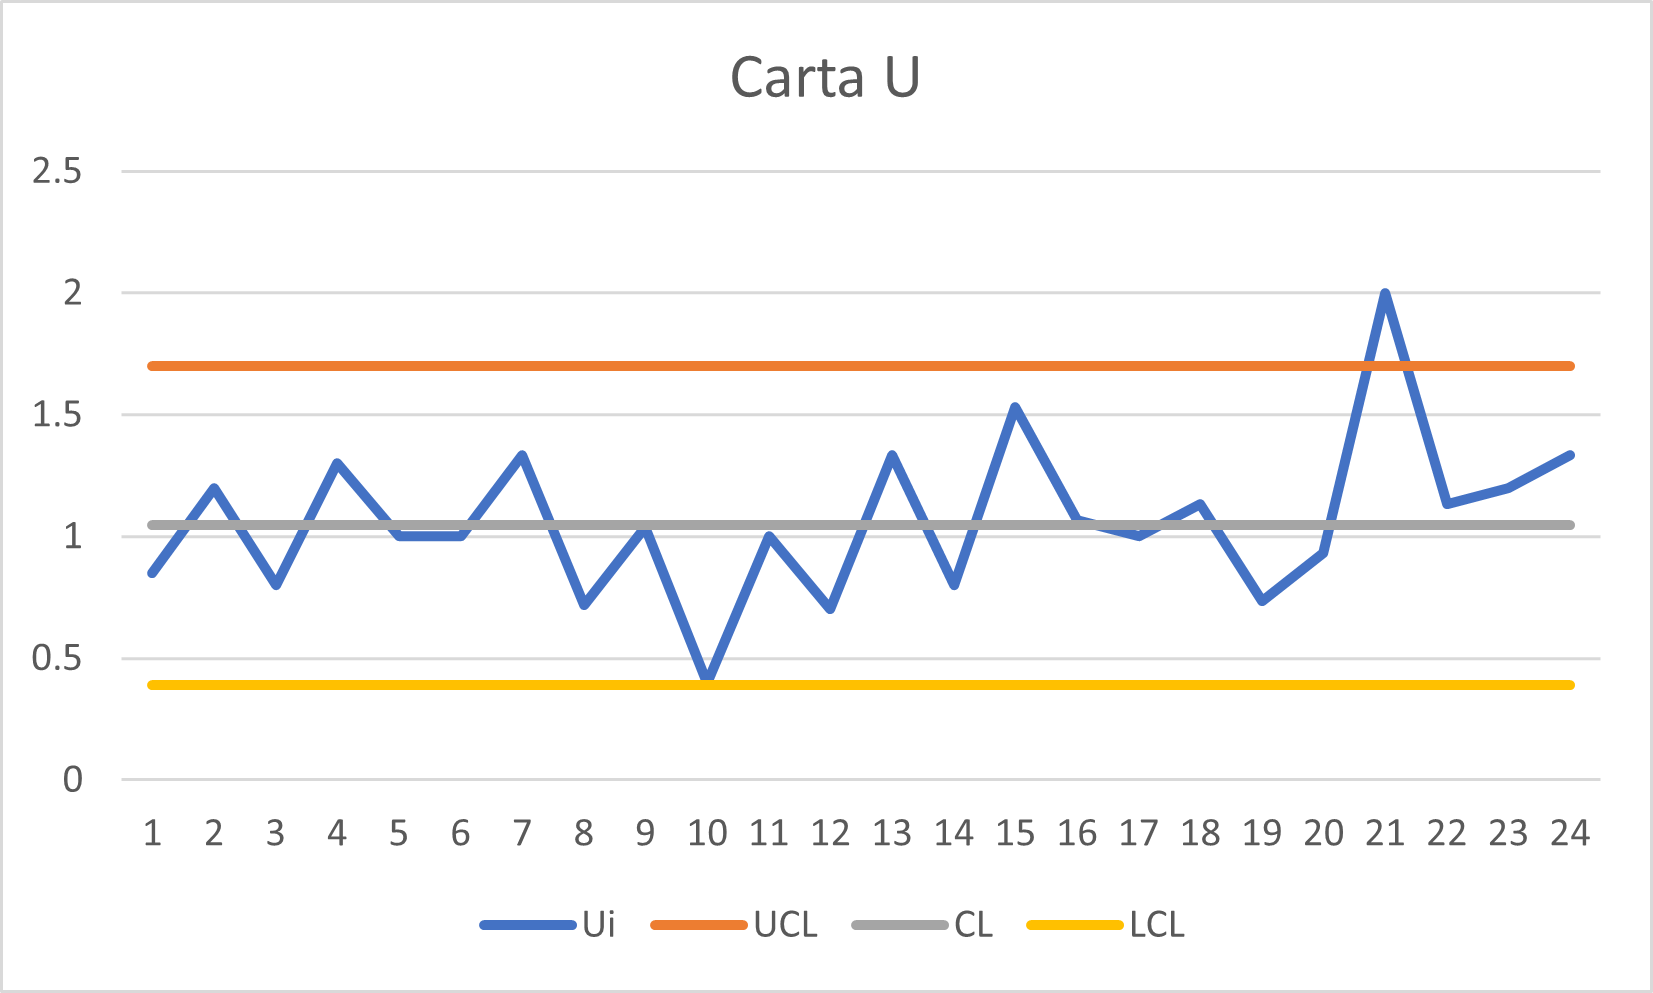
\includegraphics[width=0.6\textwidth]{GrafU.png}
	\caption[short]{Gráfico Carta U}
	\label{fig:imagen2}
  \end{figure}
  \bibliographystyle{apacite}
\nocite{*}
\bibliography{cartas-por-atributos}
\end{document}